\section{Introduction}
\label{sec:intro}

%concurrent data structures round trips
Concurrent data structure design for remote memory is hard.
Access latency to remote memory is high so round trips per
operation must be minimized to achieve efficiency.
Serialization is particularly hard because there is no
centralized serialization point to guard access to remote
memory. RDMA NIC's provide atomic verbs such as
compare-and-swap (CAS), but these are by no means a silver
bullet.  Each atomic request takes a round trip from client
to server to execute. In the best case lock/unlock requires
two round trips, if multiple locks are required, or locks
are contested the number of round trips increases.

%cpu locking vs rdma
In traditional key value stores (Memcached~\cite{memcached})
the CPU coordinates table access for read, write, and lock
instructions. In contrast RDMA based Key-value
stores~\cite{herd,erpc,pilaf} use a mixture of one-sided (no
cpu) and two-sided (cpu involved) verbs to alleviate the CPU
bottleneck. Reads are typically one sided to bypass the CPU
bottleneck~\cite{pilaf,cell} while writes are typically two
sided so memory-side CPU can orchestrate serialized
operations (e.g. locking) with main memory access latency
(50-100ns).  These small access times keep critical sections
small for CPU based locking, and dramatically increase them
for one-sided RDMA based locking schemes~\cite{clover,
sherman}.

%rdma and cuckoo hashing
In this work we examine the tradeoffs between optimistic and
lock based data structures for remote memory. Our
contribution is a new concurrent hash table design which
uses a novel cuckoo hashing algorithm. Our algorithm
(rcuckoo) is designed to enable locking and unlocking
efficiently using one-sided RDMA. In the common case our
reads execute in a single round trip, and updates to the
table are performed in two round trips. To achieve this
efficiency we make use of \textit{dependent hashing} to
increase the locality between hash location in our cuckoo
hash. Dependent hashing enables efficient reads, fast
heuristic search for open location, and efficient locking.
To achieve fast locking we make use of new RDMA NIC device
features, mainly RDMA masked CAS operations and device
mapped memory. Rcuckoo is designed with RDMA NIC's in mind
to achieve high throughput and low latency.

%%
Implement a prototype of our algorithm in python and
evaluate it in a simulator against another state of the art
remote hashing algorithm RACE. We demonstrate that in the
common case rcuckoo requires fewer round trips, and
therefore achieves lower latency and higher throughput than
race but up to a factor of 2x on YCSB workloads.



\section{Background}
\label{sec:background}

\subsection{RDMA}

\begin{figure*}[t]
    \centering
    \begin{subfigure}{0.3\linewidth}
        \includegraphics[width=0.99\linewidth]{fig/rdma_latency.pdf}
        \label{fig:rdma_latency}
        % \caption{}
    \end{subfigure}.
    \begin{subfigure}{0.3\linewidth}
        \includegraphics[width=0.99\linewidth]{fig/rdma_concur.pdf}
        % \label{fig:optimistic_failures}
        % \caption{}
    \end{subfigure}
    \begin{subfigure}{0.3\linewidth}
        \includegraphics[width=0.99\linewidth]{fig/rdma_cas_throughput.pdf}
        % \label{fig:optimistic_failures}
        % \caption{}
    \end{subfigure}
    \vspace{-1em}
    \caption{
    \textbf{(a)} CX5 RDMA latency vs message size~\cite{rdma-latency}
    \textbf{(b)} RDMA operation scalability
    \textbf{(c)} Compare and swap performance. Device memory vs main memory.
    }
    \label{fig:rdma-benchmarks}
\end{figure*}

RDMA is a networking technology which allows client machines
to directly access the memory of a remote server. RDMA is an
enabling technology for memory disaggregation as
\textit{memory servers} do not need any computation
resources (save setting up the RDMA memory initially). RDMA
is designed for extremely high throughput and low latency.
Bandwidth capabilities of RDMA NICs have increased
disproportionately to their latency improvement. The
bandwidth difference between CX3 and CX7 NICs is 10x and yet
intra rack round trips of small RDMA packets has only shrunk
by around 1.5x. Comparatively bandwidth is cheaper than
latency. ~\ref{fig:rdma-benchmarks}(a) shows the tradeoff
between NIC to NIC round trips times on CX5 RDMA NICs for
write operations. All packets up to 128 bytes have
comparable round trip latencies, and packet sizes must grow
to above 1K before the cost of the large packet exceeds the
cost of two round trips for smaller packets. In a network
with surplus bandwidth if single large messages can be used
to achieve the work of two dependent smaller messages system
latency can be improved.

One sided RDMA verbs (read, write, atomic) are used to
access remote memory without any memory side computation.
One sided verbs require RDMA reliable connections which
guarantee in-order delivery of operations enabling dependent
operations to be issued in batches. Operation throughput is
not equivalent across all verbs. Reads and writes scale
approximately linearly, however atomic operations suffer
from throughput bottlenecks at approximately half the
throughput~\cite{design-guidelines,sherman}.
Figure~\ref{fig:rdma-benchmarks}(b) shows the scalability of
these operations on CX5 NICs for 64 bit operations.

The cause of RDMA atomic throughput bottlenecks is mostly
due to PCIe round trips to host memory. NICs are forced to
use complex internal locking schemes which inspect in flight
requests across queue pairs to ensure that no dependent
operations execute concurrently. Vendors have provided small
amounts on-device memory which does not suffer this
limitation~\cite{device-memory}. Device memory access is
lower latency in general as it avoids the PCIe round trip,
and much faster for locking as the critical section is
executed entirely on the NIC~\ref{fig:rdma-benchmarks}(c)
shows the relative performance of CAS operation on device
memory vs host memory. Lock request on a single address are
3x higher throughput, and independent lock requests scale at
nearly the same rate as read and write requests.

RDMA operations are known to have limitations~\cite{prism},
pointer deference, memory allocation, and the scope of CAS
operations are the most debated. Due to fixed width CAS
operations, and no support for mutli-CAS, RDMA based
algorithms using optimistic concurrency can only update
single 64 bit values atomically. Vendors have provided
masked CAS operations~\cite{rdma-masked-cas} to set multiple
bits independently, this however is not a general solution
as it still demands data locality for items being
independently updated.


\subsection{RDMA Key-Value Stores}

Many projects have used RDMA to accelerate key-value
stores~\cite{farm,erpc,herd,mica,pilaf,cell,faast,storm,memc3}.
RDMA verb use is a matter of contention among these systems.
Typically reads are made lovelessly and directly to remote
memory, while writes use two-sided verbs and are coordinated
by the server side CPU.
%%
Far memory key-value stores have no server side CPU and must
therefore use client side synchronization to achieve
serializablity~\cite{rolex,fusee,clover,sherman,ford,race}.
These systems make use of RDMA atomic verbs for
serialization. However, the use of the atomics is highly
dependent on the key value stores under lying data
structure.

\textbf{Data Structures} - The underlying data structures of
far-memory key value stores has a large impact on the
systems performance. To perform fast reads CPU colocated
systems have used cuckoo and hopscotch
hashing~\cite{pilaf,herd,cuckoo,hopscotch}. While these
structures have fast predictable reads, they have a large
number of updates required for
insertions~\cite{pilaf,cuckoo-improvements,memc3}. These
large critical sections are amplified by far memory access
times and lead to performance bottlenecks when acquiring
locks. Recent work on remote memory data structures have
opted for optimistic concurrency~\cite{clover,race,ford}.
This strategy comes at the cost of additional round trips to
first learn up to date information about the remote
structure, and to ensure that the optimistic operation
completed successfully.

\textbf{Cuckoo hashing} is a hash table which hash constant
time reads. It uses two hash functions to determine two
possible locations at which any hashed item can reside. When
reading both locations are queried. If the item is not
found, it is not in the table. On insert, the item is placed
in the first location it hashes to. If that location is full
the item in that location is evicted and kicked to it's
second location.  This process happens iteratively for many
items. The sequence of displaced keys on an insert is called
a ~\textit{cuckoo-path}~\cite{cuckoo-improvements}. When a
loop occurs in a cuckoo path the insert fails and the table
is resized. Fill factors for cuckoo hashes can be improved
but using associative buckets for each hash index, and
shortening cuckoo paths by using BFS rather than radom
search~\cite{cuckoo-improvements}.

\section{Problems}
\label{sec:problems}

Far memory data structure design is difficult because of
it's high access latency. Operations which require
synchronization or blocking are amplified by the latency.
Operations which would be prohibitively expensive if they
were run on local DRAM can be feasible and scalable for far
memory. For example pushing complexity to the client is
often beneficial as it reduces load on the server. Examples
include caching remote data to improve optimistic
operations, making writes associative and reads large enough
to capture entire associative buckets, and adding
computation to the client to reduce contention. Here we
detail the problems and challenges of using traditional
cuckoo hashing on far memory.


\textbf{Caching:} Modifying a remote data structure requires
clients to have synchronized caches. The cache can either be
accumulated per operation and be discarded or persist across
operations.  Accumulating a cache per operation is slow,
clients must aquire locks, read, then release potentially
many times to complete an operation if the locks are fine
grained. Alternatively clients can persist a cache across
requests in the hope that it will be valid for future
operations.  Clover (a remote memory key value store) caches
pointers to values on clients to enable fast reads when
values are looked up multiple times~\cite{clover}.
Optimistic caching threads a fine line as issuing optimistic
operations which commonly fail may be worse than acquiring
the correct locks.  An ideal caching strategy would enable
clients to succeed in their operations frequently while not
requiring much overhead to maintain. 


%cuckoo hashing optimistic vs locks
\textbf{Critical Sections:} Consider executing an insert
into a concurrent cuckoo hash stored in remote memory. A
client with a cached index may have little or very stale
information about the state of the hash table. To insert the
client must gather information by reading buckets to compute
a cuckoo path. With concurrent clients this leads to a
chicken and egg problem when acquiring locks vs making
reads.

%% optimistic inserts
A client can perform inserts opportunistically by executing
lockless read to learn about the hash table, calculating a
cuckoo path, and executing a sequence of dependent CAS
operations for each step in the path. This approach is
scalable as its critical section is only the length of a CAS
instruction and is only limited by RDMA atomic operation
throughput~\cite{design-guidelines}. However, Paths can
become invalid as other clients running concurrent inserts
invalidate the paths. Figure~\ref{fig:cuckoo-problems}(a) shows the
path insertion failure rate as the number of concurrent
clients grows. This approach minimizes round trips as
dependent CAS operations can be batched thanks to in order
delivery provided by RDMA reliable connections.
Unfortunately failed inserts require additional round trips
to both fix the state of the table, and retry the
insert.\sg{Further - Issuing CAS as a batch leads to complex
path failure cases such a single element in the path failing
while others further down the path succeed. Assesing and
fixing such insertion failures without locks is very hard.}

% lock based inserts
Alternatively to get synchronized information the client can
lock the table, then issue reads. However acquiring locks
without knowledge of the table is hard. A global lock
ensures that all reads are synchronized, but bottlenecks
hash table throughput. Alternatively per bucket locks
enable high throughput but calculating which buckets to lock
requires knowledge of the table. A long cuckoo path may
require locking many buckets and many round trips to gather
information about the hash table.
%%
An ideal protocol would enable clients to perform inserts
without bottlenecks the insert performance of the hash
table, while requiring the fewest round trips to construct
and execute the cuckoo path.

% First, acquiring a lock means a round trip. If the table has
% a single lock, then a client is guaranteed to be able to
% gather all the locks it requires in a single round trip.
% However a single lock does not scale as only a single writer
% can write at a time. This matter is made worse by the fact
% that the critical section of the lock is larger in remote
% memory. Breaking the table up into subtables each with it's
% own lock has it's own problems. An insertion with a long
% path will potentially need to acquire many locks. Each of
% which requires a round trip. Therefore using fine grained
% locking increases the tables scalability but increases it's
% base case insertion time.

\textbf{Read Optimization:} Most data center workloads are
read heavy, therefore read operations should be the most
highly optimized~\cite{datacenter-workloads,facebook-memcached}. Prior
approaches such as RACE require two RDMA round trips per
read. The first is a hash index lookup, the second round
trip reads the actual key-value block. RACE must perform two
round trips because entries in the hash index are limited to
64 bits (CAS width). This is commonly not enough to store
both key and value so RACE can not inline both keys and
values in the index structure. Clover~\cite{clover} enables
single round trips reads. However under contention Clovers
reads require pointer chasing which is known to be expensive
due to each pointer resolution requiring a round
trip~\cite{clio,clover,pointer-chaising}. Ideally we would
be able to ensure that reads complete in a single round
trip.

\textbf{Duplicate Keys:} Clients may issue concurrent
inserts for the same key, given that keys may occupy
multiple location detecting and dealing with duplicate keys
is tricky while maintaining high performance. RACE requires
an extra round trip after each insert to check if a
duplicate key was inserted simultaneously~\cite{race}. An
ideal algorithm would prevent key duplication without
requiring additional overheads.


\section{Design}
\label{sec:design}

\begin{figure*}[t]
    \centering
    \begin{subfigure}{0.3\linewidth}
        \begin{align*}
            L_1 &= h_1(k) \\
            L_2 &= L_1 + h_2(k) \% f^{f + log_2(h_3(k))}
        \end{align*}
        % \caption{}
        % \label{fig:hash_factor}
    \end{subfigure}
    \begin{subfigure}{0.3\linewidth}
        \includegraphics[width=0.99\linewidth]{fig/hash_factor.pdf}
        % \label{fig:hash_factor}
        % \caption{}
    \end{subfigure}
    \begin{subfigure}{0.3\linewidth}
        \includegraphics[width=0.99\linewidth]{fig/hash_fill.pdf}
        % \label{fig:hash_fill}
        % \caption{}
    \end{subfigure}.
    \vspace{-1em}
    \caption{
    \textbf{(a)} Dependent hashing for factor $f$.
    \textbf{(b)} CDF of distances between cuckoo locations dependent hashing on different exponential factors.
    \textbf{(c)} Exponential factor relation to max fill in cuckoo hash.
    }
    \label{fig:locality-hashing}

\end{figure*}




\subsection{Locality Hashing}
Both cuckoo~\cite{cuckoo} and hopscotch~\cite{hopscotch}
hashes are optimized for reads. Cuckoo hashing ensures
constant time reads, while hopscotch hashing ensures that a
read is within a bounded range of it's hash index. Both of
these properties have been noticed by the RDMA key-value
store, and far memory communities for their fast
reads~\cite{memc3,cuckoo-improvements,pilaf,farm}.

Our approach aims to combine the bounded reads of cuckoo
hashing, with the locality properties of hopscotch hashing.
To do so we make our two hash functions \textit{dependent}
and bound the distance between cuckoo hash locations.  The
first hash function determines the location a key will be
hashed to. The second hash function determines the maximum
distance the second value can have from the first. A third
hash function determines a random location between the first
location, and the bound imposed by the second.
Figure~\ref{fig:locality-hashing}(a) shows the formula for
our dependent hashing function.

A strawman implementation of locality based hashing would
use the first hash function to find a location, and the
second to find a random location within a fixed bound. This
approach quickly leads to failed insertions. Due to the
birthday paradox the probability of a collision is high, and
on large tables the probability that one region of the hash
table will become full, and have not viable path to an open
slot is high. ~\sg{Perhaps this justifies a figure, please
advise.}.

We use a dynamic exponential bound rather than a static one.
The dynamic bound is set by raising a constant factor $f$ by
an exponent determined by a third hash function. Using the
third hash on the key we count the number of suffix zeros
and raise the constant factor by itself plus the zero count.
This distribution generates exponential distances between
hash locations at exponentially less frequency and is
tunable with the single parameter $f$.
%%
In the common case the bound is small. Exponentially few key
are spaced far apart and act as~\textit{waypoints} to other
regions of the table when constructing cuckoo paths. This
method, paired with bucket associativity enables high fill
rates while keeping the region of the table any given key
can inhabit small.

There is a tradeoff between locality and fill factor.
Figure~\ref{fig:locality-hashing}(b) illustrates how
increasing the exponential factor shifts the distribution of
distances between cuckoo hash locations.
Figure~\ref{fig:locality-hashing}(c) shows how these same
factors effect the max fill rate of the table before an item
cannot be inserted. As will be shown in the following
sections read, and insert performance improve with better
locality. Therefore fill factor and performance can be
traded off directly by changing the exponential factor. In
our evaluation we found an exponential factor of 2.3 to give
the best results in terms of end to end performance and
bandwidth consumption.


\subsection{Locking}

\begin{figure*}[t]
    \centering
    \begin{subfigure}{0.3\linewidth}
        \includegraphics[width=0.99\linewidth]{fig/optimistic_failures.pdf}
        % \label{fig:optimistic_failures}
        % \caption{}
    \end{subfigure}
    \begin{subfigure}{0.3\linewidth}
        \includegraphics[width=0.99\linewidth]{fig/insertion_span.pdf}
        \label{fig:insertion_span}
        % \caption{}
    \end{subfigure}.
    \begin{subfigure}{0.3\linewidth}
        \includegraphics[width=0.99\linewidth]{fig/buckets_per_lock_vs_locks_per_message.pdf}
        \label{fig:tbd}
        % \caption{}
    \end{subfigure}.
    \vspace{-1em}
    \caption{
    \textbf{(a)} Failure rate of optimistic cuckoo insertions.
    \textbf{(b)} CDF of cuckoo spans for dependent and independent hashing. A cuckoo span is the distance between the smallest and largest index in a cuckoo path.
    \textbf{(c)} Round trips (99th percentile) required per insert while filling a table to 100\% while varying the lock per message, and buckets per lock. \todo{subtract one from each current values include unlocks}
    }
    \label{fig:cuckoo-problems}

\end{figure*}



Traditional wisdom would suggest that because cuckoo hashing
can have long insertion paths it is a poor candidate for
remote memory. Both opportunistic, and lock based approaches
have significant drawbacks.
%%
As an example consider an opportunistic approach in which
many clients are inserting concurrently to a table. Clients
making inserts first make reads of the table to locally
calculate a cuckoo path for their insertion. After the reads
complete the client constructs a cuckoo path and starting
from the open slot issues dependent CAS requests migrating
the open slot backwards to the insertion bucket.
%%
Figure~\ref{fig:cuckoo-problems}(a) shows the failure rate
of this insertion scheme as a factor of clients running
inserts on a table with 500K entries with a bucket
associativity 8. Cuckoo paths calculated from client caches
quickly become invalid as the number of clients grows.
%%
Alternatively deadlock free lock acquisition requires more
round trips and has larger critical sections. Each lock must
be acquired in order with a dependent CAS request which
incurs an additional round trip per lock. Using course
grained locks reduces the number of acquisitions but
throttles throughput as concurrent insertions are more
likely to contend shared locks.

Locality hashing increases the probability that an insertion
path is within a small region of the hash table which in
turn increases the probability that fine grained locks will
be near one another. 
%%
Figure~\ref{fig:cuckoo-problems}(b) shows the insert span in
buckets using both dependent and independent hashing on a
table with 500K entries and an associativity of 8. A span is
calculated as the distance between the lowest index and the
highest index in a cuckoo path. Past 50\% independent
hashing spans a random range in the table (whenever a
displacement occurs on insert). With dependent locality
based hashing 95\% of inserts span less than 32 buckets, and
99\% less than 256.
%%
RDMA masked CAS operations allow a client to set a 64 bit
mask along with the new, and old values of the cas
operation. So locks can be acquired with minimal knowledge
of the remote lock table. This enables the client to
atomically set up to 64 contiguous locks independently which
dramatically reduces the round trips required to aquire
locks.

Lock granularity effects performance under contention. Using
values from Figure~\ref{fig:rdma-benchmarks}(b) if locks are
per bucket 96\% of lock acquisitions can be completed with a
single RTT masked cas. If locks span 4 buckets 99\% of
requests can be completed in a single round trip.
%%
Figure~\ref{fig:rdma-benchmarks}(c) shows the tradeoff between lock
granularity and the number of locks which can be set in a
single message with locality hashing turned on. The values
reported are the 99th percentile number of round trips
required to acquire locks up to a 90\% fill factor on a
table with 4096 entries and 8 entries per bucket, and 8
concurrent clients. The biggest factor in round trip times
is the number of locks per bucket. On the far right side of
the heatmap (512) only a single global lock exists. Further
the benefit in terms of locks per message falls off quickly
after 1. RDMA masked CAS are beneficial as they allow for
fine grained locking, but setting 3 or more locks per
message has little effect up to 90\% fill rate. Reducing
atomic operations in turn reduces the effect of the RDMA
atomic bottleneck.

Our lock table is small in comparison to the true hash
table. At it's most fine grained each lock corresponds to
one bucket (8 entries). Each lock is 1 bit, a lock table for
a 100 million entry hash table is ~160KB, with a lock
granularity of 4 buckets this drops to 40KB. This tight
layout enables us to use device mapped memory to hold our
lock table~\cite{design-guidelines,sherman}. This enables up
to 3x better throughput on contested locks (see
Figure~\ref{fig:rdma-benchmarks}(c)), and reduces latency
for locking.

\subsection{Table Design}

We design our table with flexibility in mind. Our goal is to
support inlining fixed sized keys and values in the index,
while simultaneously supporting variable sized values.
Unlike one-sided hash functions which have their index
entries limited to a CAS width~\cite{race}, rcuckoo supports
variable sized entries because updates are guarded by client
held locks rather that RDMA CAS operations. Inlining entries
has the benefit that reads require a single round trip,
their halfing their latency. Further keys can be stored
directly in the index, not just their
digests~\cite{pilaf,race}, this too removes the need to read
extent data to verify that an index entry matches it's true
key. Figure~\ref{fig:table-diagram} illustrates our table
design.  Each entry includes an extent bit to indicate if
the entry is inlined or stored in an extent. We make use of
device mapped memory on recent RDMA NIC's (ConnectX-5+) to
reduce locking latency~\cite{sherman} and enable higher
throughput. Device mapped locking avoids an expensive PCIe
round trip, and reduces on NIC blocking when acquiring
locks.


\begin{figure}[t]
    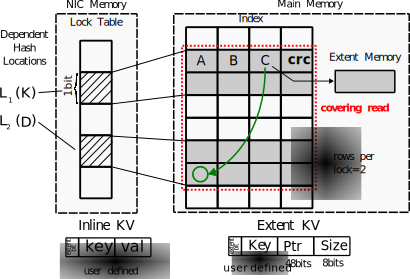
\includegraphics[width=0.99\linewidth]{fig/table-diagram.pdf}
    \caption{Rcuckoo's table design}
    \label{fig:table-diagram}
\end{figure}


\subsection{Protocol}

\begin{figure}[t]
\includegraphics[width=0.99\linewidth]{fig/message_diagram.pdf}

\caption{Rcuckoo's protocol for reads, inserts, deletes and
updates. Blue lines are index accesses, and red lines are
extent accesses. Solid lines are reads, dotted lines are
CAS, and curved dashed lines are writes.}

\label{fig:message_diagram}
\end{figure}

In this section we describe our protocol for reading,
inserting, and performing updates and deletes to an rcuckoo
hash table. Figure~\ref{fig:message_diagram} visualizes our
protocol.

\subsubsection{Reading} All reads are performed locklessly.
If keys and values are inlined clients complete reads in a
single round trip, otherwise a second round trip is required
to resolve a pointer and read the extent. 
%%
~\footnote{This design requires exactly one pointer
resolution in expectation that future RDMA NICs may provide
pointer resolution reads as a primitive~\cite{prism}}
%%
The index is modified concurrently by writes, clients must
therefore validate their reads by computing a CRC post
read~\cite{pilaf,cell}.
%%
In the base case clients compute both hash locations for a
key and issue two bucket sized RDMA read requests to the
index. As an optimization clients can perform reads using a
single packet. We define a read threshold of 512 bytes for
our clients, if two hash locations are within 512 bytes we
issue a single large read.  Approximately 60\% of keys for
64bit entries with a bucket size of 8 (see
Figure~\ref{fig:locality-hashing}(b)) fall into this
category. This has the advantage of updating the client
cache for future operations, and reduces the header
processing required by the NIC. To reduce bandwidth the size
of the threshold can be tuned down, or turned off with no
harm to correctness.

\subsubsection{Locking and unlocking}

Update, delete and insertion operations all require locks to
modify the index. Locks are acquired in incremental order
from smallest to largest to avoid deadlocks. First the list
of locks required for the operation is calculated. For
updates and deletes this requires a single lock, for insert
many locks may be required. Once the client has calculated
which buckets it needs to lock it computes a list of RDMA
masked CAS requests. If the locks required are within 64
locks of one another they are batched together into a single
masked CAS request. After the list is computed the client
issues the request for each lock one at a time. If a request
fails that request is retried until the lock is acquired.

Clients need their caches synchronized with remote memory
prior to modifying it with writes. We batch reads with lock
requests to synchronize client caches. RDMA in-order
delivery ensures that reads issued after a lock request will
be up to date, as no other client can concurrently modify
the locked index.  A spanning read is issued for each lock
request. The read covers each bucket the client locks. If a
masked CAS has three locks reads are calculated for each
bucket being locked. If the locks cover a range less than
the read threshold a single read is issued which spans all
buckets between the locks. Spanning reads are batched with
lock requests. Subsequent lock requests are issued prior to
blocking on reads.

After locks are acquired the client can execute it's
critical section. Unlock requests are the inverse CAS
operations of the lock requests. Clients issue their
critical sections as a sequence of writes, and batch unlock
operations with them. RDMA in order delivery ensures that
the unlock operations are performed after the critical
section.

\subsubsection{Updates and Deletes}

Updates and deletes are performed in a similar fashion.
First the client aquire locks for the key it will update or
delete. If the key exists the client updates it's value with
a write and then releases the locks. For updates the client
updates the value and the CRC of the index, for deletes the
index is simply set to NULL. If extents are being used
updates asynchronously write their extent data during lock
acquisition. Both updates and deletes for extents remove the
old extent data lazily. Regardless of if extents are turned
on updates and deletes are performed in two round trips.

\subsubsection{Insert}

Unlike updates and deletes inserts may span the index and
require many locks. Determining which locks to acquire is
hard as clients may have stale caches. We use a two phase
search strategy to find insertion paths. First the client
constructs a cuckoo path using it's cached index. The client
then acquires the locks for it's cuckoo path. Once the
client has it's locks thanks to the spanning reads it's
cache is fully synchronized with remote memory. A second
search is then performed using only the buckets the client
hash locked. If this search is successful the client
calculates the updates to the cuckoo path batches them as a
series of writes and issues them along with it's unlock
requests.

If the first search fails the client performs a read and
tries again. If this fails the table must be resized. The
second search may fail because the clients cache was stale
and the list of locked buckets was insufficient to perform
the insert. In this case the client releases the locks and
performs the insertion from the start again by performing an
unrestricted search on it's local cache. In the common case
insertions take two round trips. When the hash table is less
than 50\% full the probability that a cuckoo path which a
length greater than one is required is low. If extents are
used the client batches the extent write during it's locking
phase.

\textbf{Key Duplication:} Unlike RACE our algorithm can
prevent duplicate keys easily on insert~\cite{race}. RACE
requires three round trips for inserts, the third re-reads
the index to ensure no duplicates were inserted
concurrently.  Alternatively Cuckoo hashing inserts to
exactly one bucket, which is read during the lock
acquisition phase. If a duplicate key is found the client
can abort. If the bucket is full, a duplicate key may exist
in it's alternative bucket. Our clients issue a read to the
inserted keys alternative bucket during lock acquisition. If
the lock returns successfully and no duplicate exists in
either bucket then no duplicates exist as the successful
lock ensures that no other client is currently moving the
key to another location as part of a concurrent insert.


\subsubsection{A* Search} 

Locality based hashing provides us opportunities for better
search than traditional cuckoo hashing. Cuckoo hashing
insert traditionally uses random replacement~\cite{cuckoo}.
Random replacement requires little computation, however at
high fill rates it leads to long cuckoo paths which require
many locks, and reduce concurrent throughput. BFS search
finds the shortest path and has been demonstrated to
increase system throughput with fine grained
locking~\cite{cuckoo-improvements}.  BFS is
computationally intensive. Locality based hashing enables us
to leverage more efficient search strategies. Because
locality hashing increases the probability that a cuckoo
hashing location is close we can use an informed search
algorithm to find open slots close to bucket a key hashes
to. 
%%
In the case of BFS the target bucket is unknown, therefore
all paths must be explored. We use A* search, an algorithm
which takes a goal location, and a distance heuristic as
input. A* is known to find shortest paths in much better
average case times than BFS. A* requires two additional
inputs, a distance heuristic and a goal location.

\textbf{Goal location}: Locality hashing increases the
probability that an open slot near the insertion target
location can terminate a cuckoo path. Our algorithm collects
open slots near the original hash location as candidate goal
locations. By default we set the number of candidate goal
locations to 5. Goal locations are collected by starting at
the $h_1(k)$ location and iterating through the hash
table both forward and backwards through the table one index
at a time. Buckets with open slots are added to the
candidate list until the limit is reached. 

% \todo{I could
% improve this search time by tracking the list of open
% buckets and using binary search on them.}.

\textbf{Search Heuristic}: A* requires a heuristic for
distance which is a strict underestimate of the true
distance to a goal. A typical heuristic for search is the
euclidean distance between two points. A * guarantees that
if the search heuristic is a strict underestimate of the
true distance to the goal then the path found will be the
shortest path. In our case we use the distance between a
goal state and a current state is unknown as the distance
between any two buckets is the result of our locality
hashing function which has no upper bound. However we can
estimate the distance between two buckets by using the mean
distance of our locality hash function. This approach does
not guarantee that we find the shortest path, however it
does find short paths in the common case, and results in
very short search times.

\section{Implementation} We implement our algorithm in
Python and emulate client based RDMA using a custom built
simulator consisting of 1k lines of code. 

\textbf{Simulator:} Our simulator is event based and does
not emulate network transit time, processing time, or failed
packets. Clients, memory, and switches are modeled as finite
state machines, and the network as FIFO queues. Events are
scheduled randomly, multiplexing clients, memory, and the
network. RDMA verbs are modeled as function pointers with
arguments passed by the client.

\textbf{Rcuckoo} is implemented in 1.2k lines of
python. We implement our own version of approximate A* with
the use of python's standard heap library for priority
queuing. Clients store complete copies of the remote hash
table index locally. We do not model the hash table extent
in simulation all table accesses are inlined. In practice
for better resource utilization cached pages of the index
could be released using LRU. 

\textbf{RACE~\cite{race}} has no publicly available
implementation. Therefore we implemented our own version of
RACE by closely following it's protocol as described in it's
paper.  We only model the RACE index. In cases where
blocking calls are made to RACE's extent we assume they
succeed and simply reissue a read to the index to model the
round trip incurred by the extent lookup. We model RACE's
blocking behavior exactly in this way. We reached out to
RACE's authors to check our implementation's correctness and
were able to correlate our fill factor results with theirs.

\section{Evaluation}
\label{sec:eval}

\begin{figure*}[ht]
    \includegraphics[width=0.99\linewidth]{fig/hero_ycsb_throughput.pdf}
    \caption{race vs rcuckoo simulated throughput \todo{rerun ycsb-b numbers don't look quite right}}
    \label{fig:ycsb_throughput}
\end{figure*}

\begin{figure*}[ht]
    \includegraphics[width=0.99\linewidth]{fig/hero_ycsb_fill_latency.pdf}
    \caption{race vs rcuckoo workload fill latency}
    \label{fig:ycsb_fill_latency}
\end{figure*}

\begin{figure}[ht]
    \includegraphics[width=0.99\linewidth]{fig/hero_ycsb_fill_ops_bw.pdf}
    \caption{YCSB-A workload messages and bandwidth per operation as a function of fill factor}
    \label{fig:ycsb_fill_ops_bw}
\end{figure}

\begin{figure}[ht]
    \includegraphics[width=0.99\linewidth]{fig/search_dependence.pdf}

    \caption{Round trips per insert operation compared
    across search functions and hash functions. Dependent
    hash functions with A* have the shortest search
    times.~\todo{latest numbers for A* are counter intuitive
    - dig into}}

    \label{fig:search_dependence}
\end{figure}

Our evaluation is run entirely in simulation. The goal of
our evaluation is to demonstrate the practicality of rcuckoo
by showing through simulation that it supports low latency
and high throughput operations. We measure blocking round
trip's as a proxy for latency. To approximate throughput we
measure the total number of blocking round trips required to
fill the table, and divide by the number of concurrent
clients. All of our evaluations are carried out on hash
tables with buckets of size 8, and key-value pairs with
32bit keys and 16bit values. On hash tables with 1 million
entries. Rcuckoo is set with a read threshold of 512 bytes.

In each experiment clients operate on a shared remote hash
table, but insert and read independent sets of keys. Using
independent keys prevents clients from reading absent keys,
and inserting duplicate keys.  However it does not prevent
interference due to hash collisions or conflicting cuckoo
paths.


\subsection{System Performance}

\textbf{Throughput:} Figure~\ref{fig:ycsb_throughput} shows
the throughput of RACE vs rcuckoo for YCSB workloads. YCSB-W
is a 100\% write workload. YCSB-A is a 50\% read 50\% write
workload. YCSB-B is 95\% read and 5\% write, and YCSB-C is
100\% read.  In each experiment clients fill the hash table
from empty to 90\% full. For read only workloads the hash
table is first filled to 90\% and then clients read from the
table.  Note that on large tables rcuckoo inserts scale
almost linearly as the number of path collisions on inserts
remains low due to the short cuckoo range.  Read heavy
workloads (ycsb-b, c) have the highest throughput due to
fewer round trips. In the case of ycsb-c rcuckoo achieves 2x
the read throughput of RACE.

\textbf{Latency:} Rcuckoo's operation latency is not static
across fill factors. Because cuckoo paths are likely to be
longer at higher table saturations inserts are more likely
to require more round trips when obtaining locks. We measure
the round trips as a proxy for latency at incremental fill
factors. In each experiment the table is filled to the
specified fill factor and requests are executed until the
table reaches an additional 5\% fill or in the case of read
only 500k. Each experiment is run with 128 clients.
requests are issued. 
%%
Figure~\ref{fig:ycsb_fill_latency}, shows the average
operation latency for each workload. Here average RTT is the
average between both reads, and writes. RACE incurs
additional round trips from reading from it's extent and
from verifying it's successful inserts. RACE has very few
collisions as its critical section for insertion is the
duration of a single RDMA CAS. Few of RACE's inserts fail
and it retains near constant latency for read and writes
across all fill factors. The same is true for rcuckoo reads
which remain at a single round trip. Rcuckoo inserts are
subject to additional round trips as the table fills.  Most
additional round trips are caused by locks being spaced
further than the span of an RDMA CAS on the lock table. Some
are caused by contention. The small improvement of ycsb-a
and ycsb-b over ycsb-w inserts are due to reduced write
contention from the workload.

\textbf{Bandwidth, and messages:} Rcuckoo design trades off
bandwidth for latency by increases the size of reads for all
operations. We measure the effect of fill factor on the
bandwidth and messages required per operation with the same
experiment used to measure latency.
Figure~\ref{fig:ycsb_fill_ops_bw} shows how rcuckoo and
RACE's messages and bandwidth respond to fill factor. At low
fill rates (less than 50\%) rcuckoo uses less bandwidth per
operation and less messages per operation than RACE. Above
50\% collisions in the hash table increase the cost of
insertions. While the size of the cuckoo path does not
directly relate to the number of round trips, it does
directly relate to messages. High fill factors nearly double
the number of insert messages required to perform insertions
with rcuckoo, and bandwidth can increase by up to a factor of
4. \todo{In the future we could perform very large writes to
reduce the number of messages at the cost of more
bandwidth.}

\textbf{Locks per message and independence:} Hash function
locality hash a major impact in rcuckoo's performance.
Acquiring locks can only be done in a few round trips when
the locks are clustered together tightly in the lock table.
Furthermore, the search function used to determine the
cuckoo path has a large impact on the locality of the locks
necessary to lock the path. We evaluate dependent hashing
and independent hashing as well as random and a* search. We
measure the number of round trips required for each control
as a function of the number of locks which can be acquired
per round trip.

Figure~\ref{fig:search_dependence} shows the performance
improvements gained by both locality hashing and A* search.
In this experiment the table is filled from 0 to 90\% full
with a ycsb-w workload. We measure the 99th percentile of
round trips for these workloads. Random search with
independent hashing leads to a large number of round trips
as locks are scattered throughout the table. RDMA masked CAS
operation do little here to reduce the round trips as they
can rarely aquire more than one lock in a round trip. With
dependent hashing and random search RDMA CAS operation are
almost sufficient to reduce round trips, however the absolute
number of locks required per insert is high which leads to
greater contention. A* search with dependent hashing has
cuckoo paths that are both short, and clustered together.



\subsection{Search Performance:}

\todo{\textbf{A* search vs BFS:} We compare the performance of A*
vs BFS for locally computed insertions. A* performance
directly effects system throughput as this algorithm is run
twice on every insert.}

\todo{\textbf{Hashing Algoritms:} Rcuckoo hashing requires
executing many hash compuations. We evaluate our A* search
alorithm abolute performacne on various hash functions and
show how this values effect our overall fill factors.}

\subsection{Read Threshold Performance} 

\todo{Show how it reduces messages per operation. This is not that
important of an experiment as I can't show the latency
overhead of two batched messages vs one at the moment.}
%%


\section{Conclusion}
\label{sec:conclusion}

In this work we design and implement a lock based cuckoo
hash for remote memory. Using dependent hashing, a carefully
designed locking protocol, and the latest RDMA NIC features
we achieve common case operations of 2 round trips, and
lockless reads in a single round trip. We demonstrate that
these algorithmic advantages lead to better practical
performance by simulating hash table workloads and showing
throughput and latency benefits of up to 2x over state of
the art far memory hash tables.
